\subsection{The Radical of a Module}

DEFINITION 1. --- Let A be a ring. The radical of an A-module M is the submodule defined as the intersection of the maximal submodules of M (VIII, p.~48, Definition 2) or, equivalently, the set of elements of M annihilated by every homomorphism from M to a simple A-module.

In the remainder of this chapter, we denote the radical of an A-module M by \(\mathfrak{R}_{\mathrm{A}}(\mathrm{M})\) or simply \(\mathfrak{R}(\mathrm{M})\) .

Let A be a ring. The radical of an A-module M is reduced to 0 (in which case we say, by abuse of language, that M is without radical) if and only if there exist a family \((\mathrm{S}_{i})_{i\in\mathrm{I}}\) of simple A-modules and a family \((f_{i})_{i\in\mathrm{I}}\) of A-linear mappings \(f_{i}:M\to S_{i}\) such that we have \(\cap_{i\in\mathrm{I}}\mathrm{Ker}(f_{i})=0\) . This is equivalent to M being isomorphic to a submodule of a product of simple A-modules.

Examples. --- 1) Let \(\mathfrak{a}\) be a left ideal of A. The radical of the A-module \(\mathrm{A}_s / \mathfrak{a}\) is equal to \(\mathfrak{a}' / \mathfrak{a}\) , where \(\mathfrak{a}'\) is the intersection of the maximal left ideals of A containing \(\mathfrak{a}\) . In particular, the radical of the Z-module \(\mathbf{Z}\) is reduced to 0, and that of the Z-module \(\mathbf{Z} / p^n\mathbf{Z}\) is equal to \(p\mathbf{Z} / p^n\mathbf{Z}\) for every prime number \(p\) and every integer \(n \geqslant 1\) .

\begin{enumerate}
\def\labelenumi{\arabic{enumi})}
\setcounter{enumi}{1}
\tightlist
\item
  Let A be a principal ideal domain that is not a field, and let K be its field of fractions. As a K-module, K is without radical. Let us prove that the radical of K, viewed as an A-module, is equal to K; equivalently, we must prove that every A-linear mapping f from K to a simple A-module S is zero. By VII, §4, No.~8, p.~25, we may assume that S is equal to \(\mathrm{A}/(\pi)\) , where \(\pi\) is an irreducible element of A. We have \(f(x) = f\left(\pi \frac{x}{\pi}\right) = \pi f\left(\frac{x}{\pi}\right) = 0\) for every \(x \in \mathrm{K}\) because \(\pi \mathrm{S} = 0\) .
\end{enumerate}

PROPOSITION 1. --- Let M and N be A-modules and f a homomorphism from M to N. We have \(f(\mathfrak{R}(M)) \subset \mathfrak{R}(N)\) , and we even have equality if f is surjective and the kernel of f is contained in the radical of M.

Let g be a homomorphism from N to a simple A-module; then \(\mathfrak{R}(M)\) is contained in the kernel of \(g \circ f\) , so that \(f(\mathfrak{R}(M))\) is contained in the kernel of g. We therefore have \(f(\mathfrak{R}(M)) \subset \mathfrak{R}(N)\) . Now suppose that f is surjective and that its kernel is contained in \(\mathfrak{R}(M)\) . Let y be an element of \(\mathfrak{R}(N)\) , and let x be an element of the inverse image of y. If g is a homomorphism from M to a simple A-module S, then its kernel contains the radical of M, hence the kernel of f.~Since the homomorphism f is surjective, there exists a homomorphism h from N to S such that \(g = h \circ f\) . Since \(y = f(x)\) belongs to \(\mathfrak{R}(N)\) , we have \(h(f(x)) = 0\) , that is, \(g(x) = 0\) ; thus x belongs to \(\mathfrak{R}(M)\) , which proves the inclusion \(\mathfrak{R}(N) \subset f(\mathfrak{R}(M))\) .

COROLLARY 1. --- Let M be an A-module and N a submodule of M.

\begin{enumerate}
\def\labelenumi{\alph{enumi})}
\item
  We have \(\Re (\mathrm{N})\subset \Re (\mathrm{M})\cap \mathrm{N}.\)
\item
  We have \((\Re (\mathrm{M}) + \mathrm{N}) / \mathrm{N}\subset \Re (\mathrm{M} / \mathrm{N})\) . If N is contained in \(\Re (\mathrm{M})\) , then we have the equality \(\Re (\mathrm{M} / \mathrm{N}) = \Re (\mathrm{M}) / \mathrm{N}\)
\item
  The module \(\mathrm{M} / \Re (\mathrm{M})\) is without radical. If the module \(\mathrm{M} / \mathrm{N}\) is without radical, then we have \(\Re (\mathrm{M})\subset \mathrm{N}\) .
\end{enumerate}

Assertion a) follows from Proposition 1 applied to the canonical injection from N to M, and assertion b) follows from Proposition 1 applied to the canonical mapping from M to M/N. From b), we deduce that M/N is without radical if \(N = \Re(M)\) and that we have \(\Re(M) \subset N\) if M/N is without radical.

\pandocbounded{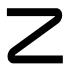
\includegraphics[keepaspectratio]{images/part001_4ea857d0.jpg}}

It follows from Example 1 that there can exist submodules N containing \(\Re(\mathrm{M})\) such that the radical of M/N is not zero.

COROLLARY 2. --- Let \((\mathrm{M}_{i})_{i\in\mathrm{I}}\) be a family of A-modules, P its product, and S its direct sum. We have \(\Re(\mathrm{P})\subset\prod_{i\in\mathrm{I}}\Re(\mathrm{M}_{i})\) and \(\Re(\mathrm{S})=\bigoplus_{i\in\mathrm{I}}\Re(\mathrm{M}_{i})\) .

For \(i \in I\) , let \(\pi_{i}\) be the projection with index i from P to \(M_{i}\) . By Proposition 1, we have \(\pi_{i}(\mathfrak{R}(P)) \subset \mathfrak{R}(M_{i})\) for every \(i \in I\) ; this proves the first assertion. We have \(S \subset P\) , hence

\[
\mathfrak {R} (S) \subset S \cap \mathfrak {R} (P) \subset S \cap \prod_ {i \in I} \mathfrak {R} (M _ {i}) = \bigoplus_ {i \in I} \mathfrak {R} (M _ {i}).
\]

Moreover, we have \(M_{i} \subset S\) and therefore \(\Re(M_{i}) \subset \Re(S)\) for every \(i \in I\) , and consequently \(\oplus_{i \in I} \Re(M_{i}) \subset \Re(S)\) .

There exist families of modules such that the radical of the product is not isomorphic to the product of the radicals (Exercise 3 of VIII, p.~166).

PROPOSITION 2. --- Let M be a finitely generated A-module.

\begin{enumerate}
\def\labelenumi{\alph{enumi})}
\item
  If \(\mathbf{M}\) is not reduced to 0, then we have \(\Re (\mathbf{M})\neq \mathbf{M}\) .
\item
  If N is a submodule of M such that \(\mathrm{N} + \Re(\mathrm{M}) = \mathrm{M}\) , then we have N = M.
\end{enumerate}

Let N be a proper submodule of M. By Proposition 3 of VIII, p.~49, there exists a maximal submodule L of M containing N. We have \(\mathrm{N} + \Re(\mathrm{M}) \subset \mathrm{L}\) , and a fortiori \(\mathrm{N} + \Re(\mathrm{M}) \neq \mathrm{M}\) . This proves b); the specific case N = 0 gives assertion a).

COROLLARY. --- Let M be an A-module, \((x_{i})_{i\in\mathbb{I}}\) a generating family of M, and x an element of M. The following properties are equivalent:

\begin{enumerate}
\def\labelenumi{(\roman{enumi})}
\item
  We have \(x \in \Re(\mathbb{M})\) .
\item
  Every submodule N of M such that \(\mathrm{N} + \mathrm{A}x = \mathrm{M}\) is equal to M.
\item
  For every family \((a_{i})_{i\in\mathrm{I}}\) of elements of A, the family \((x_{i}+a_{i}x)_{i\in\mathrm{I}}\) generates the A-module M.
\item
  \(\Rightarrow\) (ii): Suppose that x belongs to \(\Re(\mathrm{M})\) . Let N be a submodule of M such that \(N + Ax = M\) . We have \(N + \Re(M) = M\) ; hence the A-module M/N is equal to its radical (Corollary 1, b) of Proposition 1). Since it is monogenous, it is zero (Proposition 2), and we have M = N.
\item
  \(\Rightarrow\) (iii): Let \((a_{i})_{i\in\mathrm{I}}\) be a family of elements of A. Denote by N the submodule of M generated by the family \((x_{i}+a_{i}x)_{i\in\mathrm{I}}\) . We have \(x_{i}\in N+Ax\) for every \(i\in I\) , hence \(N+Ax=M\) . If property (ii) holds, then N is equal to M.
\item
  \(\Rightarrow\) (i): Suppose that x does not belong to \(\Re(\mathrm{M})\) . Then there exists a maximal submodule N of M that does not contain x. Since N is maximal, we have \(N + Ax = M\) ; each of the elements \(x_{i}\) can therefore be written as \(y_{i} - a_{i}x\) with \(y_{i} \in N\) and \(a_{i} \in A\) . The family \((x_{i} + a_{i}x)_{i \in I}\) is contained in N, hence does not generate M.
\end{enumerate}

PROPOSITION 3. --- a) A semisimple module is without radical.

\begin{enumerate}
\def\labelenumi{\alph{enumi})}
\setcounter{enumi}{1}
\tightlist
\item
  A module is semisimple and finitely generated if and only if it is without radical and Artinian.
\end{enumerate}

By definition, the radical of a simple module is reduced to 0. If the module M is semisimple, then it is the direct sum of a family \((\mathrm{S}_{i})_{i\in\mathrm{I}}\) of simple submodules, and we have \(\mathfrak{R}(\mathrm{M})=\bigoplus_{i\in\mathrm{I}}\mathfrak{R}(\mathrm{S}_{i})\) by Corollary 2 of Proposition 1 above, hence \(\mathfrak{R}(\mathrm{M})=0\) .

If, moreover, M is finitely generated, then it is Artinian by Proposition 10 of VIII, p.~71.

Conversely, suppose that M is Artinian and without radical. By VIII, p.~2 applied to the set of maximal submodules of M, there exists a finite family \((\mathrm{N}_{i})_{i\in\mathrm{I}}\) of maximal submodules of M whose intersection is reduced to 0. Then M is isomorphic to a submodule of \(\bigoplus_{i\in\mathrm{I}}(\mathrm{M}/\mathrm{N}_{i})\) . Therefore, it is semisimple and has finite length, and is a fortiori finitely generated.

